\documentclass[fontsize=12pt,paper=a4,twoside]{scrartcl}

% SWP-Präambel
% C 2003-2021 Sebastian Offermann, Rainer Koschke, Karsten Hölscher
% In Zeilen 41 und 42 sind jeweils die aktuellen Semester-Daten einzutragen.

\usepackage[utf8]{inputenc}     % Kodierung der Tex-Datei
\usepackage[T1]{fontenc}        % Korrekte Ausgabe von Sonderzeichen (Umlaute)
\usepackage[ngerman]{babel}     % Deutsche Einstellungen [ab \begin{document}]

\usepackage{bibgerm}            % Bibliographie
\usepackage{fancyhdr}           % obere Seitenränder gestalten
\usepackage{float}              % Floats Objekte mit [H] festsetzen
\usepackage{graphicx}           % Graphiken als jpg, png etc. einbinden
\usepackage{moreverb}           % zusätzliche verbatim-Umgebungen
\usepackage{pdflscape}          % PDF-Support für landscape
\usepackage[final]{pdfpages}    % Externe PDFs einbinden
\usepackage{stmaryrd}           % zusätzliche Symbole
\usepackage{supertabular}       % Tabellen über Seitenränder hinaus
\usepackage{tabularx}           % Tabellen mit vorgegebener Breite
\usepackage{url}                % setzt URLs schön mit \url{http://bla.laber.com/~mypage}

%%% Die Reihenfolge der folgenden Pakete muss beibehalten werden:
%%% varioref, hyperref, cleveref, bookmark
% Verweise innerhalb des Dokuments schick mit " ... auf Seite ... "
% automatisch versehen. Dazu \vref{labelname} benutzen
\usepackage[ngerman]{varioref}  % [vor hyperref für korrekte Verweise]
\usepackage[colorlinks=true, pdfstartview=FitV, linkcolor=blue,
            citecolor=blue, urlcolor=blue, hyperfigures=true,
            pdftex=true]{hyperref} % [vor bookmark wegen der Optionen]
\usepackage[ngerman]{cleveref}
\usepackage{bookmark}

\hyphenation{Arbeits-paket}     % Trennungsregeln

%%% Definitionen
\newcommand{\grad}{\ensuremath{^{\circ}} }
\renewcommand{\strut}{\vrule width 0pt height5mm depth2mm}
\newcommand{\gq}[1]{\glqq{}#1\grqq{}}
\newcommand{\skipInput}[1]{}

%%% Semesterkonstanten
\newcommand{\sem}{WiSe}%{SoSe}
\newcommand{\jahr}{2022/23} %2017/2018

\newif\iftoc
\tocfalse % für kleine Abgaben kein Inhaltsverzeichnis nötig
%\toctrue % für größere Abgaben mit Inhaltsverzeichnis

\newcommand{\highlight}[1]{\textcolor{blue}{\textbf{#1}}}
\newcommand{\swp}{Software-Projekt}
\newcommand{\semester}{\sem\ \jahr}

%%% Formatierungsanpassungen
% Damit Latex nicht zu lange Zeilen produziert:
\sloppy
%Uneinheitlicher unterer Seitenrand:
%\raggedbottom

% Kein Erstzeileneinzug beim Absatzanfang
% Sieht aber nur gut aus, wenn man zwischen Absätzen viel Platz einbaut
\setlength{\parindent}{0ex}

% Abstand zwischen zwei Absätzen
\setlength{\parskip}{1ex}

% Seitenränder für Korrekturen verändern
\addtolength{\evensidemargin}{-1cm}
\addtolength{\oddsidemargin}{1cm}

\bibliographystyle{gerapali}

\newcommand\documentTitle{Bitte documentTitle festlegen!}
\newcommand\groupName{Bitte groupName festlegen!}
% swpdocument verwendet die Werte von documentTitle und groupName,
% entsprechend sollten diese vorher umgesetzt werden; sonst wird eine
% Erinnerungsmeldung an der entsprechenden Stelle im Dokument platziert
% 1. Parameter: Euer/Eure Tutor:in, z. B. {Kim Harrison}
% 2. Parameter: Abgabedatum, z. B. {05. April 2063}
% 3. Parameter: Versionsnummer, z. B. {1.1}
% 4.-9. Parameter: jeweils Name und (Uni-)Email-Adresse jedes 
%                 Gruppenmitglieds; mit einem & getrennt, z. B.
% {Robin Cowl & roco@uni-bremen.de}
% Besteht die Gruppe aus weniger als 6 Personen, so werden die 
% übrigen Parameter leer gelassen: {}
\newcommand \swpdocument[8] {
% Lustige Header auf den Seiten
  \pagestyle{fancy}
  \setlength{\headheight}{70.55003pt}
  \fancyhead{}
  \fancyhead[LO,RE]{\swp{}\\%
                    \semester{}\\%
                    \documentTitle}
  \fancyhead[LE,RO]{Seite \thepage\\%
                    \slshape \leftmark\\%
                    \slshape \rightmark}

% Lustige Header nur auf dieser Seite (Titelseite)
  \thispagestyle{fancy}
  \fancyhead[LO,RE]{ }
  \fancyhead[LE,RO]{Universität Bremen\\%
                    FB 3 -- Informatik\\%
                    Tutor: #1}
  \fancyfoot[C]{}

% Start Titelseite
  \vspace{3cm}
  \begin{minipage}[H]{\textwidth}
    \begin{center}
      \bfseries \Large \swp{} -- \semester{}\\
      \smallskip
      \small 03-IBGP-SWP\\
      \vspace{3cm}
    \end{center}
  \end{minipage}
  \begin{minipage}[H]{\textwidth}
    \begin{center}
      \vspace{1cm}
      \bfseries {\Large \documentTitle}\\
      \vspace{3ex}
      $<$\groupName$>$\\%
      \vfill
    \end{center}
  \end{minipage}
  \vfill
  \begin{minipage}[H]{\textwidth}
    \begin{center}
      \sffamily
      \begin{tabular}{lr}
        #3 \\
        #4 \\
        #5 \\
        #6 \\
        #7 \\
        #8 \\
      \end{tabular}
      \\[22mm]
      \itshape Abgabe: #2\\ ~
    \end{center}
  \end{minipage}
% Ende Titelseite

\iftoc
%\iffalse
% Start Inhaltsverzeichnis
\newpage
  \thispagestyle{fancy}
  \fancyhead{}
  \fancyhead[LO,RE]{\swp{}\\%
                    \semester{}\\%
                    \documentTitle}
  \fancyhead[LE,RO]{Seite \thepage\\%
                    \slshape \leftmark\\~}
  \fancyfoot{}
  \renewcommand{\headrulewidth}{0.4pt}
\tableofcontents
% Ende Inhaltsverzeichnis
\fi

% Header für alle weiteren Seiten
\newpage
  \fancyhead[LE,RO]{Seite \thepage\\%
                    \slshape \leftmark\\%
                    \slshape \rightmark}

}


\usepackage[shortlabels]{enumitem}
\graphicspath{{./images/}}
%
% Und jetzt geht das Dokument los....
%
\begin{document}
\renewcommand\documentTitle{Anwendungsfälle}
\renewcommand\groupName{KarteikartenAG}
\swpdocument{Rodrigue Wete Nguempnang}{13. November 2022}%
            {Mert As & meras@uni-bremen.de}%
            {Tom Beuke & tombeuke@uni-bremen.de}%
            {Efe Carkcioglu & efe1@uni-bremen.de}%
            {Nadja Cordes & ncordes@uni-bremen.de}%
            {Ole-Niklas Mahlstädt & olma@uni-bremen.de}%
            {Henry Zöllner & henry5@uni-bremen.de}%

\section{Detaillierte Anwendungsfälle}\label{sec:detailliert:Anwendungsfälle}

\subsection{Neue Karte erstellen}
\textbf{Name:}
\begin{itemize}
	\item N1 Karteikarte anlegen
\end{itemize}
\textbf{Akteure:}
\begin{itemize}
	\item Lehrer Leo
	\item Studi Susi
\end{itemize}
\textbf{Vorbedingungen:}
\begin{itemize}
	\item Das System ist gestartet.
	\item Leo hat sich angemeldet.
	\item Es existiert bereits mindestens eine Kategorie
\end{itemize}
\textbf{Nachbedingungen:}
\begin{itemize}
	\item Sie hat erfolgreich eine neue Karte erstellt.
	\begin{itemize}
		\item Es gibt keine Priorität für die Karte
	\end{itemize}
\end{itemize}
\textbf{Regulärer Ablauf:}
\begin{enumerate}
	\item Leo klickt auf den Button Add. (Siehe Abbildung \ref{fig:cards-1})
	\item Fenster für Neue Karte Erstellen wird geöffnet. (Siehe Abbildung \ref{fig:cards-2})
	\item Leo wählt die Kategorie aus, in der sie die Karte erstellen möchte.
	\item Leo wählt die Typ der Karte aus.
	\item Leo füllt die Informationen für beide Seiten der Karte aus.
	\item Leo klickt auf den Button Add. (Siehe Abbildung \ref{fig:cards-3})
	\item Fenster schließt sich.
	\item Die Karte wurde erfolgreich erstellt. (Siehe Abbildung \ref{fig:cards-4})
\end{enumerate}
\textbf{Alternative:}
\begin{itemize}
	\item Leo bricht den Prozess ab, bevor die Karte erstellt wird.
	\item Leo fügt Schlagwort für die Karte hinzu.
\end{itemize}
\textbf{Fehler-/Ausnahmefälle mit deren Nachbedinungen:}
\begin{itemize}
	\item Leo wählt keinen Kartentyp
	\begin{itemize}
		\item Es wird eine entsprechende Warnung angezeigt.
		\item Leo kann die Karte nicht erstellen.
	\end{itemize}
	\item Leo wählt keine Kategorie aus.
	\begin{itemize}
		\item Es wird eine entsprechende Warnung angezeigt.
		\item Leo kann die Karte nicht erstellen.
	\end{itemize}
	\item Leo hat eine oder beide Kartenseiten leer gelassen.
	\begin{itemize}
		\item Es wird eine entsprechende Warnung angezeigt.
		\item Leo kann die Karte nicht erstellen.
	\end{itemize}
\end{itemize}

\subsection{Kategorien \& Karteikästen}
\textbf{Name:}
\begin{itemize}
	\item N26 Karteikasten aus mehreren Kategorien erstellen
\end{itemize}
\textbf{Akteure:}
\begin{itemize}
	\item Lehrer Leo
	\item Studi Susi
\end{itemize}
\textbf{Vorbedingungen:}
\begin{itemize}
	\item Die Anwendung ist gestartet
	\item Es existiert bereits mindestens eine Kategorie
	\item Die ausgewählten Kategorien enthalten mindestens eine Karte
\end{itemize}
\textbf{Regulärer Ablauf:}
\begin{enumerate}
	\item Nutzer (,,Lehrer Leo`` oder ,,Studi Susi``) wechselt zur Kategorie-Übersicht (Siehe Abbildung \ref{fig:cat_deck_1})
	\item Nutzer wählt eine/mehrere Kategorie(n) aus (Siehe Abbildung \ref{fig:cat_deck_2})
	\item Nutzer führt die Aktion ,,Karteikasten`` auf der Kategorie-Auswahl aus (Siehe Abbildung \ref{fig:cat_deck_3})
	\item Nutzer wechselt damit in eine Ansicht zur Karteikasten-Bearbeitung (Siehe Abbildung \ref{fig:cat_deck_4})
	\item Nutzer gibt dem neuen Karteikasten einen Namen (Siehe Abbildung \ref{fig:cat_deck_5})
	\item Nutzer ändert ggf. weitere Einstellungen (Lernsystem, initiale Kartenreihenfolge)
	\item Nutzer bestätigt aktuellen Zustand und erstellt den Karteikasten
\end{enumerate}
\textbf{Varianten:}
\begin{itemize}
	\item Nutzer wählt in der Karteikasten-Bearbeitungs-Übersicht einzelne Karteikarten dazu/ab
	\item Nutzer fügt aus der Karteikasten-Bearbeitungs-Übersicht weitere Kategorien hinzu/ab
	\item Nutzer bricht den Prozess ab, bevor der Karteikasten erstellt wird
	\item Nutzer betreibt Client mit Server und wählt in den Karteikasten-Einstellungen ,,privat/öffentlich`` aus
\end{itemize}
\textbf{Nachbedingungen:}
\begin{itemize}
	\item Es wurde ein neuer Karteikasten angelegt (Siehe Abbildung \ref{fig:cat_deck_6})
	\begin{itemize}
		\item Taucht in der Karteikasten-Übersicht auf
		\item Hat initial keinen Lernfortschritt
	\end{itemize}
\end{itemize}
\textbf{Fehler-/Ausnahmefälle mit deren Nachbedingungen:}
\begin{itemize}
	\item Die ausgewählten Kategorien enthalten keine Karteikarten
	\begin{itemize}
		\item es wird eine entsprechende Warnung angezeigt
		\item man kann nicht bestätigen und Karteikasten erstellen
	\end{itemize}
	\item Der ausgewählte Karteikastenname ist bereits vergeben
	\begin{itemize}
		\item entsprechender Fehler wird angezeigt
		\item man kann nicht bestätigen und Karteikasten erstellen
	\end{itemize}
\end{itemize}

%%%%%%%%%%%%%%%%%%%%%%%%%%%%%%%%%%%%%%%%%%%%%%%%%%%%%%%%%%%%%%%%%%%%%%%%
\section{Anwendungsfälle}

{ \em Auflistung und kurze Beschreibung aller relevanten
	Anwendungsfälle. Dies soll einen Überblick über alle Anwendungsfälle
	geben, die zur Erreichung der Mindestanforderungen nötig sind. Optionale
	Anwendungsfälle können hier zusätzlich hinzugefügt werden.
}
\subsubsection{Akteure:}
Unser Karteikartensystem hat vier Akteure.
\begin{itemize}
	\item \textbf{Schüler Sam}: Nutzt das Karteikartensystem zum Lernen von Karteikästen, die sein Lehrer erstellt.
	\item \textbf{Lehrer Leo}: Nutzt das Karteikartensystem, um Karteikästen zu erstellen und diese mit seinen Schülern zu teilen.
	\item \textbf{Studi Susi}: Nutzt das Karteikartensystem eigenständig und erstellt und lernt Karten.
	\item \textbf{Admin Anton}: (Serverfunktionen) Nutzt die Grundfunktionen des Systems und kann darüber hinaus weitere Anpassungen vornehmen.
\end{itemize}

\subsubsection{Generelle Anwendungsanfälle:}
 Akteur Nutzer: Fasst die Akteure \textit{Lehrer Leo, Schüler Sam, Studi Susi} und \textit{Admin Anton} in \textit{Generelle Anwendungsfälle} zusammen.

\textbf{Karteikarten}
\begin{enumerate}[label={N\arabic*}]
	\item Karteikarte anlegen: Der Nutzer legt ein neue Karteikarte an.
	\item Karteikarte löschen: Der Nutzer löscht eine bestehende Karteikarte.
	\label{N2}
	\item Karteikarte bearbeiten: Der Nutzer bearbeitet den Inhalt einer Karteikarte.
	\label{N3}
	\begin{enumerate}[label*={-\arabic*}]
		\item Karteikartentyp: Der Nutzer wählt einen Karteikartentyp für eine Karteikarte aus.
		% multiplechoicetest, truefalsetest, texttest, imagetest, 3dtest
		\begin{enumerate}[label*={-\arabic*}]
			\item Karteikartentyp Ankreuztest: Der Nutzer wählt als Kartentyp Ankreuztest aus.
			\item Karteikartentyp Wahr/Falsch Test: Der Nutzer wählt als Kartentyp Wahr/Falsch Test aus.
			\item Karteikartentyp Texteingabe Test: Der Nutzer wählt als Kartentyp Texteingabe aus.
			\item Karteikartentyp Bild Test: Der Nutzer wählt als Kartentyp Bild Test aus (Die Antwort ist dann eine hochzuladene Graphik).
			\item Karteikartentyp Bildbeschreibung: Der Nutzer wählt als Kartentyp Bildbeschreibung aus (Die Antwort ist dann eine Graphik mit interaktiven Elementen, z.B. zu füllende Textfelder).
			\item Karteikartentyp Audio Test: Der Nutzer wählt als Kartentyp Audio Test aus (Die Frage ist eine kleine Audiosequenz).
		\end{enumerate}
		\item Karteikarte bewerten: Der Nutzer bewertet die Karte.
		\item Karteikarten Frage bearbeiten: Der Nutzer bearbeitet die Frage einer Karteikarte.
		\item Karteikarten Antwort bearbeiten: Der Nutzer bearbeitet die Antwort einer Karteikarte.
		\item Begriffe auf Karteikarte verlinken: Der Nutzer verlinkt einen Begriff auf einer Karteikarte. Sowohl zu anderen Karteikarten als auch zu Links im Internet.
		\item Karteikarte Kategorie(n) zuordnen: Der Nutzer ordnet eine bestehende Karteikarte einer oder mehreren bestehenden Kategorie(n) zu.
		\item Karteikarte Suchbegriffe zuordnen: Der Nutzer ordnet einer Karteikarte einen oder mehrere Suchbegriff(e) zu.
		\item Karteikarte Schlagwörter zuordnen: Der Nutzer ordnet einer Karteikarte einen oder mehrere Schlagwörter zu.
	\end{enumerate}

	\item Karteikarte als PDF exportieren: Der Nutzer exportiert eine/mehrere Karteikarte(n) als PDF-Dokument.
	\label{N4}
	\item Karteikarte als JSON exportieren: Der Nutzer exportiert eine/mehrere Karteikarte(n) als JSON
	\label{N5}
	\item Karteikarte als JSON importieren: Der Nutzer importiert eine/mehrere Karteikarte(n), die als JSON vorliegen.
	\item Karteikarte als XML exportieren: Der Nutzer exportiert eine/mehrere Karteikarte(n) als XML
	\label{N7}
	\item Karteikarte als XML importieren: Der Nutzer importiert eine/mehrere Karteikarte(n), die als XML vorlieren.

	\item (Zusatz) Karteikartenerstellzeitpunkt: Zu jeder Karteikarte wird der Erstellzeitpunkt gespeichert.
	\item (Zusatz) Karteikartensichtbarkeit: Der Nutzer markiert eine Karteikarte als privat / öffentlich sichtbar.
	\item (Zusatz) Karteikarten mit Audioinhalt aufzeichnen: Der Nutzer nimmt eine kurze Audiosequenz (z.B. Aussprache eines Wortes) auf und fügt sie einer Karteikarte zu.
\end{enumerate}

\textbf{Kategorien}
\begin{enumerate}[resume, label={N\arabic*}]
	\item Kategorie anlegen: Der Nutzer legt eine neue Kategorie an.
	\item Kategorie löschen: Der Nutzer löscht eine bestehende Kategorie.
	\item Kategorie bearbeiten: Der Nutzer bearbeitet Eigenschaften einer Kategorie
	\begin{enumerate}[label*={-\arabic*}]
		\item Kategorie Bezeichnung: Der Nutzer setzt einen Namen für eine Kategorie
		\item Kategorie Polyhierarchie: Der Nutzer stellt eine Verbindung zwischen Kategorien her, indem er diese einander unter-/überordnet.
		\label{N14-2}
	\end{enumerate}
	\item Kategorien anzeigen: Der Nutzer lässt sich die bestehenden Kategorien in einer Übersicht anzeigen.
	\item Kategorie-Übersicht verändern: Der Nutzer ändert die Kategorie-Übersicht.
	\begin{enumerate}[label*={-\arabic*}]
		\item Kategorie-Übersicht sortieren: Der Nutzer sortiert die angezeigten Kategorien (reverse-) alphabetisch.
		\item Kategorie-Übersichts Polyhierarchie: Der Nutzer lässt sich alle unter-/übergeordneten Kategorien anzeigen.
	\end{enumerate}
	\item Kategorie auswählen: Der Nutzer wählt eine/mehrere Kategorien aus (markieren)
	\item Kategorie Auswahl-Aktionen: Der Nutzer führt eine Aktion auf den ausgewählten Kategorien aus (löschen (\ref{N2}), bearbeiten (\ref{N3}), unter-/überodnen (\ref{N14-2}), Karteikasten erstellen (\ref{N26}), exportieren (\ref{N4},\ref{N5},\ref{N7}))
\end{enumerate}

\textbf{Glossar/Liste}
\begin{enumerate}[resume, label={N\arabic*}]
	\item Karteikarten anzeigen: Der Nutzer listet sich alle Karteikarten in einer Übersicht auf.
	\item Karteikartenansicht verändern: Der Nutzer ändert die Darstellung, Sortierung oder Filterung der Karteikarten-Liste.
	\begin{enumerate}[label*=-\arabic*]
		% sortieren
		\item Glossar sortieren alphabetisch: Der Nutzer sortiert das Glossar in (reverse-) alphabetischer Reihenfolge.
		\item (Zusatz) Glossar sortieren Erstellzeitpunkt: Der Nutzer sortiert das Glossar nach (reverse-) Erstellzeitpunkt.
		\item (Zusatz) Glossar sortieren Karteikasten-Anzahl: Der Nutzer sortiert das Glossar nach der Anzahl der Karteikästen, in der sich die Karten befinden (bzw. reverse).
		\item (Zusatz) Glossar sortieren Kartentyp: Der Nutzer sortiert das Glossar nach dem Kartentyp (bzw. reverse).
		\item (Zusatz) Glossar sortieren Antworttext: Der Nutzer sortiert das Glossar (reverse-) alphabetisch nach dem Antworttext.
		% filtern
		\item Glossar filtern nach Kategorien: Der Nutzer filtert das Glossar nach einer/mehreren Kategorie(n).
		\item Glossar filtern nach Tags: Der Nutzer filtert das Glossar nach einem/mehreren Tag(s).
		\item Glossar filtern nach Suchbegriffen: Der Nutzer filtert das Glossar nach einem/mehreren Suchbegriff(en)
		% anzeigen
		\item Glossar Frage-Spalte ein-/ausblenden: Der Nutzer blendet die Frage-Spalte ein oder aus. % sollte das überhaupt möglich sein?
		\item Glossar Antwort-Spalte ein-/ausblenden: Der Nutzer blendet die Antwort der Karten ein oder aus.
		\item Glossar Kartentyp-Spalte ein-/ausblenden: Der Nutzer blendet den Kartentyp der Karten ein oder aus.
		\item Glossar Erstellzeitpunkt-Spalte ein-/ausblenden: Der Nutzer blendet den Erstellzeitpunkte der Karten ein oder aus.
	\end{enumerate}
	\item Karten auswählen: Der Nutzer wählt eine/mehrere Karten in der Übersicht aus (markieren).
	\item Kartenauswahl bearbeiten: Der Nutzer bearbeitet die ausgewählten Karten (siehe \ref{N3}).
	\item Kartenauswahl löschen: Der Nutzer löscht die ausgewählten Karten (siehe \ref{N2}).
	\item Kartenauswahl exportieren: Der Nutzer exportiert die ausgewählten Karten (siehe \ref{N4},\ref{N5},\ref{N7})

	%\item (Zusatz) Suchfunktion: Der Nutzer kann seine Karten nach dem Fragetext durchsuchen. % bereits in Filtern nach Suchbegriffen enthalten.
\end{enumerate}

\textbf{Lernen/Karteikasten}
\begin{enumerate}[resume, label={N\arabic*}]
	\item Karteikasten einzelne Kategorie: Der Nutzer erstellt einen Karteikasten mit Karten aus einer Kategorie.
	\item Karteikasten mehrere Kategorien: Der Nutzer erstellt einen Karteikasten mit Karten aus mehreren Kategorien.
	\label{N26}
	\item Karteikasten bearbeiten: Der Nutzer bearbeitet einen Karteikasten.
	\item Lernsystem: Der Nutzer wählt eine Lernmethode aus.
	\begin{enumerate}[label*=-\arabic*]
		\item Nutzung Leitner Methode: Das Leitner-System wird zum Lernen ausgewählt
		% Je nach Bewertung (pflicht) wird die Karte früher/später das nächste Mal vorgelegt.
		\item Nutzung Bewertungs-Methode: Der Nutzer wählt unser Lernsystem ,,Bewertung`` aus (je nach 5-Sterne-Bewertung der Karten (pflicht) wird sie schneller/später wieder vorgelegt)
		% Je nach Antwort-Zeit wird entschieden wie schnell die Karte erneut gelernt werden muss.
		\item Nutzung Timing-Methode: Der Nutzer wählt unser Lernsystem ,,Timing`` aus (je nach Beantwortungszeit wird die Karte schneller/später wieder vorgelegt, nur für \textit{Ankreuztest} und \textit{Wahr/Falsch} empfohlen)
		\item Neue Lernmethoden erstellen: Der Nutzer erstellt ein neues Lernsystem.
	\end{enumerate}
	\item Kartenreihenfolge: Der Nutzer wählt die initiale Kartenreihenfolge aus.
	\begin{enumerate}[label*=-\arabic*]
		\item Alphabetische Reihenfolge: Die Karten werden alphabetisch beim Lernen sortiert.
		\item Zufällige Reihenfolge: Die Karten werden zufällig beim Lernen sortiert.
    \end{enumerate}
	\item (Client/Server) Karteikasten privat/öffentlichen stellen: Der Client wählt aus ob der Karteikasten auf dem Server für andere Nutzer sichtbar sein soll.
	\label{N30}
	\item Kasten Lernen: Der Nutzer wählt einen Karteikasten aus und startet, den Einstellungen des Kastens entsprechend, den Lernvorgang.
	\item Lernvorgang unterbrechen: Der Nutzer unterbricht das Lernen des Karteikartens.
	\item Lernvorgang fortsetzen: Der Nutzer setzt einen unterbrochenen Lernvorgang fort.
	\item Lernfortschritt: Der Nutzer sieht sich den aktuellen Lernfortschritt eines Karteikasten an.
	\item Antwort prüfen: Der Client prüft die Antwort (ggf. gegenüber Server)
	\item (Zusatz) Status der Karteikarten: Jede Karte im Karteikasten hat einen Status, der eingesehen werden kann (Neu / Gelernt / Wiederholen) abhängig von der Lernmethode.
	\item (Zusatz) Karteikastenübersicht: Jeder Karteikasten hat eine eigene Übersicht mitsamt Status und Lernerfolg seiner Karten.
	\item (Zusatz) Karteikasten löschen: Karteikästen können gelöscht werden. Die Karten selber sind von der Löschung nicht betroffen.
\end{enumerate}
\textbf{Generelle Einstellungen}
\begin{enumerate}[resume, label={N\arabic*}]
	\item Dunkelmodus einstellen: Der Nutzer wählt im Client den Dunkelmodus aus.
	\item Hellmodus einstellen: Der Nutzer wählt im Client den Hellmodus aus.
	\item Sprache als Deutsch einstellen: Der Nutzer wählt Deutsch als Anzeigesprache des Clients aus.
	\item Sprache als Englisch einstellen: Der Nutzer wählt Englisch als Anzeigesprache des Clients aus.
\end{enumerate}

\subsubsection{Server-Client-Betrieb}
\textbf{Client-Einstellungen}
\begin{enumerate}[resume, label={N\arabic*}]
	\item Server auswählen/verbinden: Der Nutzer wählt im Client den Server aus, mit dem er sich verbinden will.
	\item Authentifizierung gegenüber Server: Der Nutzer meldet sich mit seinen Logindaten beim Server an.
	\item Abmeldung vom Server: Der Nutzer meldet sich vom Server ab.
	\item Karteikarten/Kästen downloaden: Der Nutzer downloaded Karteikarten/Kästen vom Server.
	\item Lernfortschritt synchronisieren: Der Nutzer synchronisiert seinen Lernfortschritt mit dem Server (falls offline weitergelernt wurde)
\end{enumerate}

\textbf{Server (Admin Anton)}
\begin{enumerate}[label={A\arabic*}]
	\item Server starten: Der Nutzer startet den Server.
	\item Auswahl Veröffentlichung: Der Nutzer wählt aus welche Karteikarten, Kategorien bzw. Karteikästen veröffentlicht werden sollen (\ref{N30}).
	\item Benutzer anlegen: Der Nutzer legt für externe Clients einen neuen Benutzer-Account an.
	\item Benutzer Anmeldung: Externe Nutzer können sich mit den angelegten Accounts authentifizieren.
	\item Neue Karte erstellen: Der Server speichert die erstellte Karte in der Datenbank.
	\item Karte bearbeiten: Der Server aktualisiert die bearbeitete Karte in der Datenbank.
	\item Karte löschen: Der Server löscht die ausgewählte Karte aus der Datenbank.

	\item Port Konfigurieren: Der Admin kann über die Konfigurationsdatei den Serverport ändern.
	\item Serverpräfix (HTTP) Konfigurieren: Der Admin kann den URL Präfix des Servers ändern, falls sich dieser hinter einem Proxy befindet.
	\item Anzahl der Loginversuche Konfigurieren: Der Admin kann die Anzahl der erlaubten anmeldeversuche festlegen
	\item Login timeout Konfigurieren: der Admin kann die wartezeit nach $n$ Loginversuchen festlegen.
	\item Manuelles Registrieren Konfigurieren: Der Admin kann entscheiden, ob sich User ihren Account selbst erstellen dürfen.
	\item Einträge in der Datenbank bearbeiten, anlegen/löschen: Der Admin kann mittels eines Tools die Datenbank manuell bearbeiten.
\end{enumerate}


%%%%%%%%%%%%%%%%%%%%%%%%%%%%%%%%%%%%%%%%%%%%%%%%%%%%%%%%%%%%%%%%%%%%%%%%
\clearpage
\section{Anhang: Weitere detaillierte Anwendungsfälle}
\subsection{Zur Einzelkartenansicht wechseln}
\textbf{Akteure:}
\begin{itemize}
	\item Lehrer Leo
	\item Studi Susi
\end{itemize}
\textbf{Vorbedingungen:}
\begin{itemize}
	\item Das System ist gestartet.
	\item Leo ist angemeldet und möchte seine bereits erstellten Karteikarten einsehen.
	Er glaubt, dass er sich bei der Karteikarte \dq Bundesländer Deutschland\dq bei der Antwort vertippt hat und möchte diese nachträglich einsehen und ggfs. anpassen, bevor er dazu einen Karteikasten für seinen Schüler Sam erstellt.
\end{itemize}
\textbf{Nachbedingungen:}
\begin{itemize}
	\item Die Karte ist in der Detailansicht geöffnet.
	\item Oder: Karte ist nicht vorhanden
\end{itemize}
\textbf{Regulärer Ablauf:}
\begin{enumerate}
	\item Leo öffnet sein Karteikartenglossar.
	\item Er scrollt durch sein Glossar und sucht nach der Karte.
	\item Er entdeckt die gewünschte Karte und markiert sie. (Siehe Abbildung \ref{fig:card_overview})
	\item Er klickt auf den Button \dq Einzelkartenansicht\dq. (Siehe Abbildung \ref{fig:edit_view})
	\item Er kann die Karte samt Details in einem neuen Fenster einsehen und bekommt dort alle Bearbeitungsoptionen der Karten zur Auswahl. (Siehe Abbildung \ref{fig:detail_view})
\end{enumerate}
\textbf{Alternative:}
\begin{itemize}
	\item Zu 3. Da er die Karte auf Anhieb nicht findet, filtert er durch die Suchwörter mittels Eingabe von \dq Bundesländer Deutschland\dq nach der gewünschten Karte.
	\item Zu 3. Die gewünschte Karte existiert nicht. Leo legt stattdessen eine neue über den Button \dq Karte anlegen\dq an.
\end{itemize}

\subsection{Sprache auf Englisch umstellen}
\textbf{Akteure:}
\begin{itemize}
	\item Schüler Sam
	\item Studi Susi
	\item Lehrer Leo
	\item Admin Anton
\end{itemize}
\textbf{Vorbedingungen:}
\begin{itemize}
	\item Das System ist gestartet.
	\item Das System ist auf Deutsch (bzw. nicht Englisch) gestellt.
\end{itemize}
\textbf{Nachbedingungen:}
\begin{itemize}
	\item Er hat die App Sprache erfolgreich von Deutsch auf Englisch geändert.
\end{itemize}
\textbf{Regulärer Ablauf:}
\begin{enumerate}
	\item Sam klickt auf den Button Settings.
	\item Weitere Funktionen von Settings werden angezeigt. (siehe Abb. \ref{fig:settings})
	\item Sam bringt sein Mauszeiger zu Sprachen.
	\item Weitere Funktionen von Sprachen werden angezeigt.
	\item Sam klickt auf den Button Englisch.
	\item Die Sprache wurde auf Englisch umgestellt.
\end{enumerate}
\textbf{Alternative:}
\begin{itemize}
	\item Er hat nicht genug Deutschkenntnisse, um das Wort ,,Sprachen`` zu verstehen. Deswegen bringt er seinen Mauszeiger nicht zu Sprachen und kann den Button ,,Englisch'' nicht finden. Die Sprache wird nicht geändert.
\end{itemize}


\clearpage
\section{Anhang: Bilder}

\begin{figure}[h!]
	\caption{Karte hinzufügen}
	\label{fig:cards-1}
	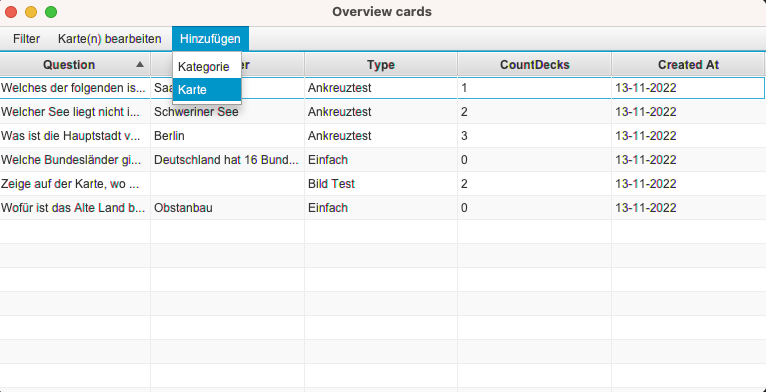
\includegraphics[width=\textwidth]{cards-1.png}
\end{figure}
\begin{figure}[h!]
	\caption{Karte muss ausgefüllt werden}
	\label{fig:cards-2}
	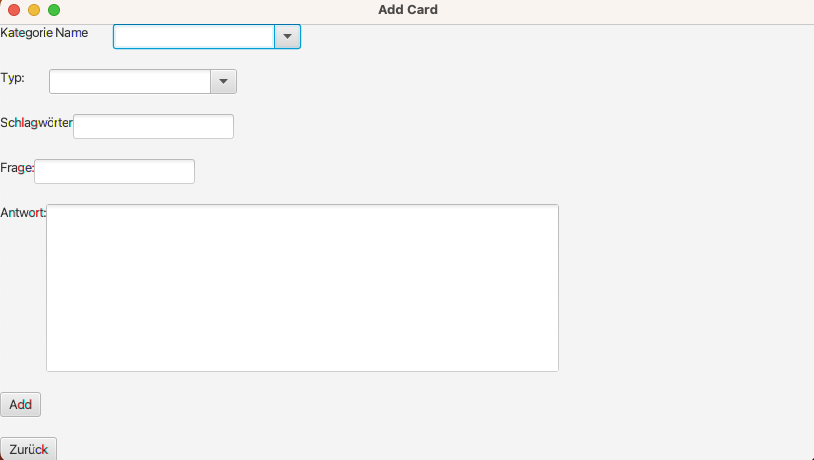
\includegraphics[width=\textwidth]{cards-2.png}
\end{figure}
\begin{figure}[h!]
	\caption{Karte ist ausgefüllt}
	\label{fig:cards-3}
	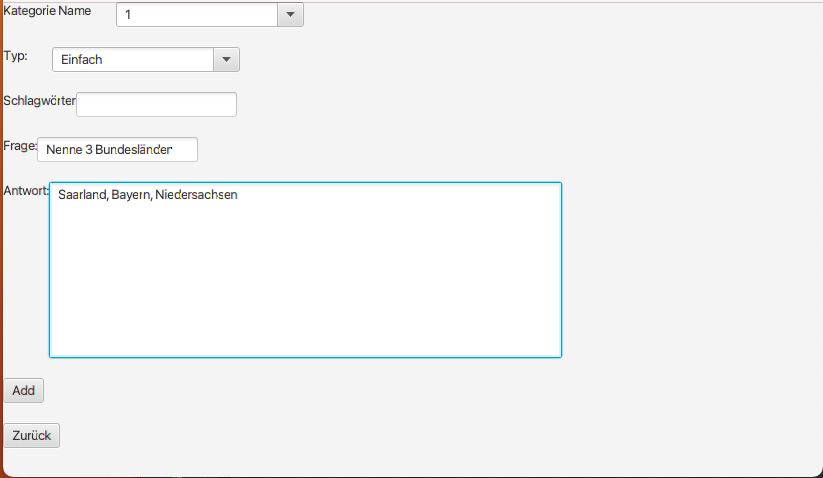
\includegraphics[width=\textwidth]{cards-3.png}
\end{figure}
\begin{figure}[h!]
	\caption{Karte in der Übersicht}
	\label{fig:cards-4}
	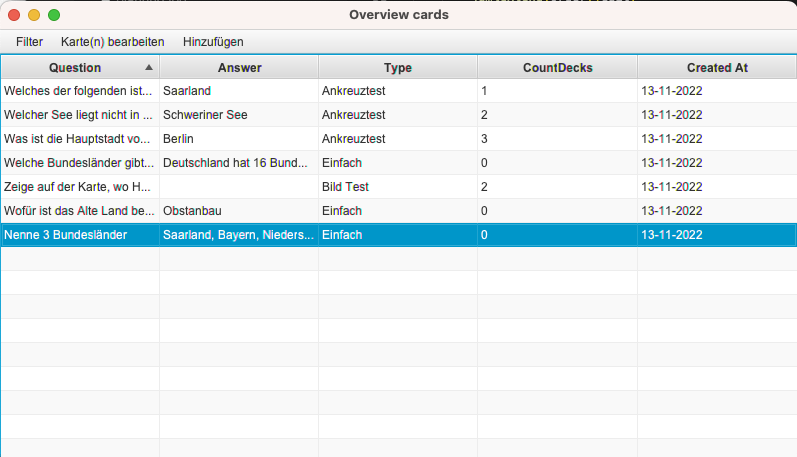
\includegraphics[width=\textwidth]{cards-4.png}
\end{figure}

\begin{figure}
	\centering
	\caption{Kategorie-Übersicht}
	\label{fig:cat_deck_1}
	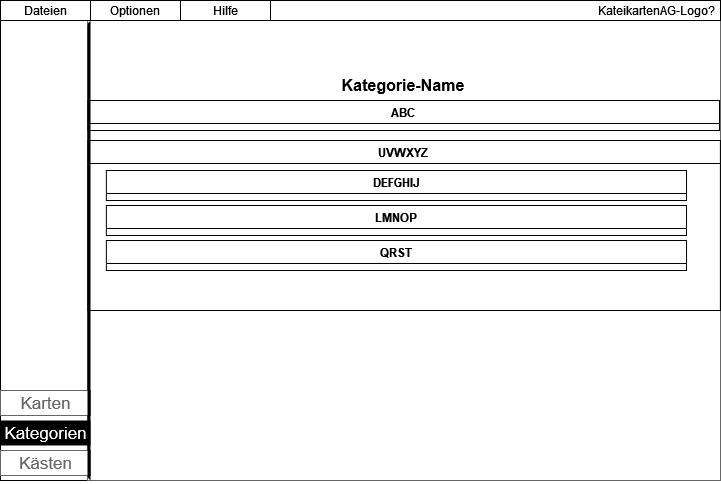
\includegraphics[width=0.9\textwidth]{mockup_categories_deck_1.png}
\end{figure}
\begin{figure}
	\centering
	\caption{Kategorien in der Übersicht auswählen}
	\label{fig:cat_deck_2}
	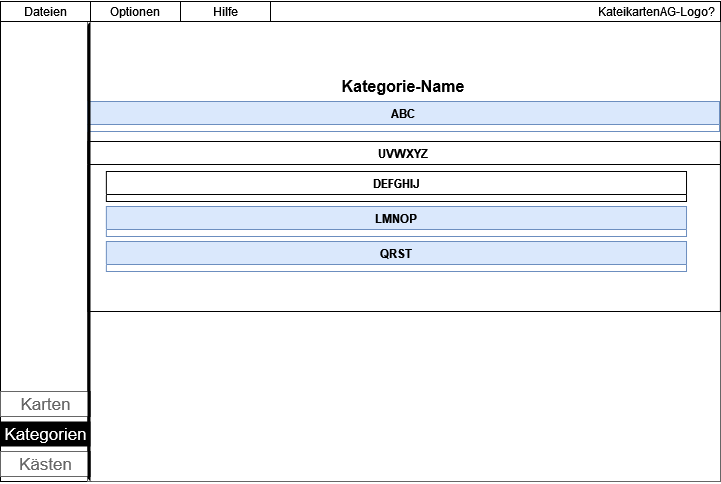
\includegraphics[width=0.9\textwidth]{mockup_categories_deck_2.png}
\end{figure}
\begin{figure}
	\centering
	\caption{Rechtsklick-Menü auf ausgewählte Kategorien}
	\label{fig:cat_deck_3}
	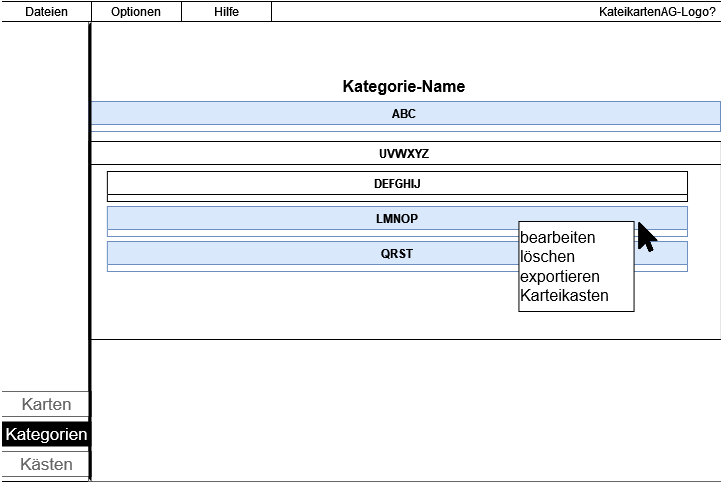
\includegraphics[width=0.9\textwidth]{mockup_categories_deck_3.png}
\end{figure}
\begin{figure}
	\centering
	\caption{Karteikasten bearbeiten (Standardeinstellungen)}
	\label{fig:cat_deck_4}
	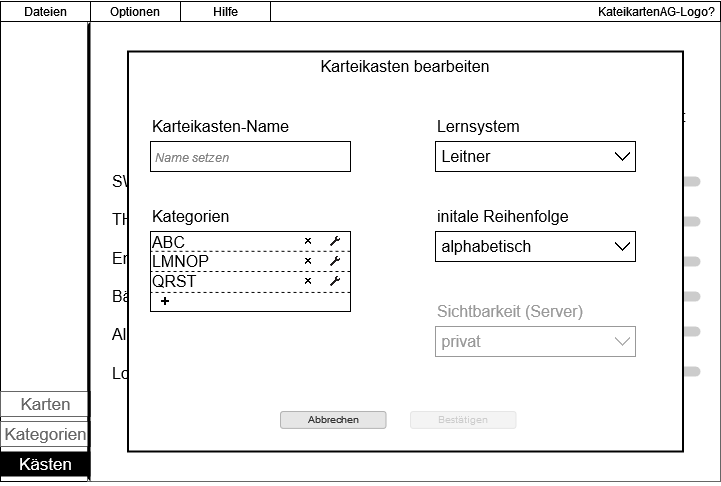
\includegraphics[width=0.9\textwidth]{mockup_categories_deck_4.png}
\end{figure}
\begin{figure}
	\centering
	\caption{Karteikasten bearbeiten mit Namen}
	\label{fig:cat_deck_5}
	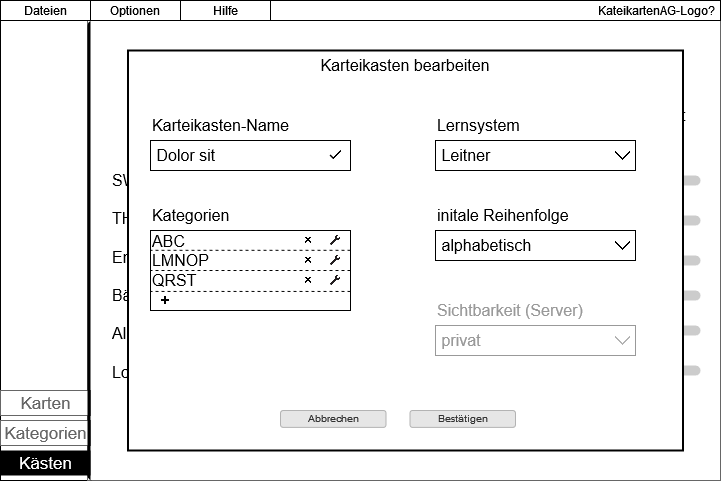
\includegraphics[width=0.9\textwidth]{mockup_categories_deck_5.png}
\end{figure}
\begin{figure}
	\centering
	\caption{Karteikasten-Übersicht}
	\label{fig:cat_deck_6}
	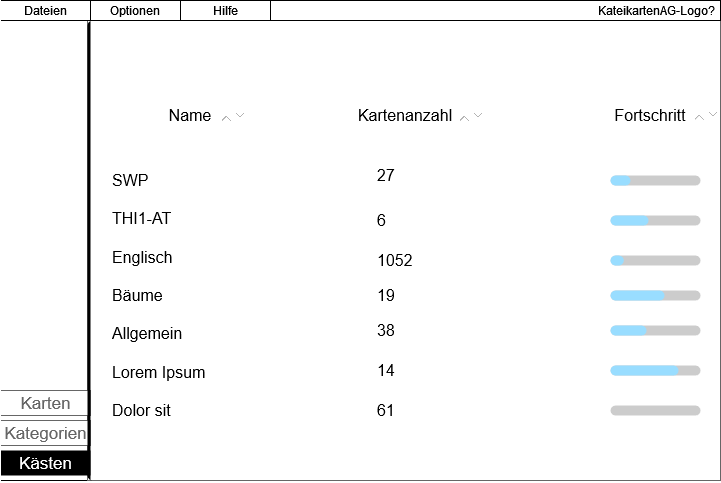
\includegraphics[width=0.9\textwidth]{mockup_categories_deck_6.png}
\end{figure}

\begin{figure}
	\caption{Kartenübersicht}
	\label{fig:card_overview}
	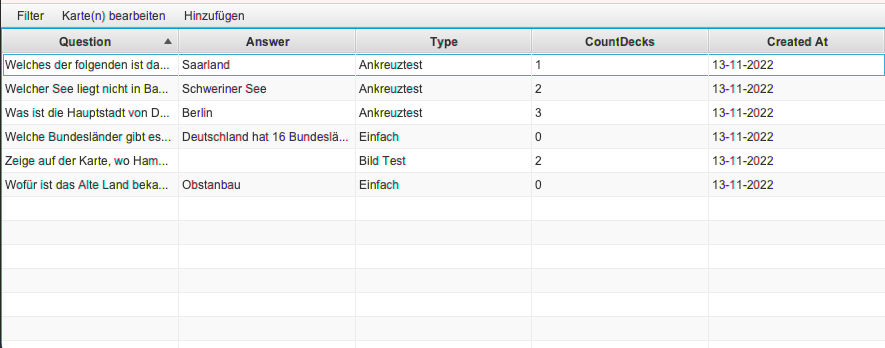
\includegraphics[width=\textwidth]{overview-details1.png}
\end{figure}
\begin{figure}
	\caption{Ansicht bearbeiten (Einzelkartenansicht)}
	\label{fig:edit_view}
	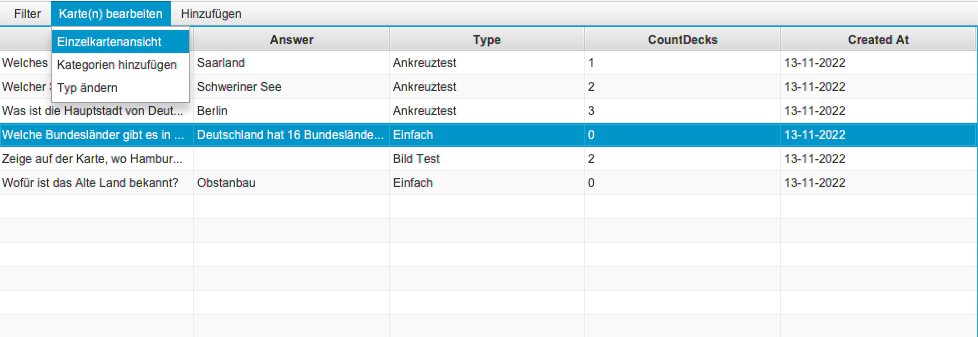
\includegraphics[width=\textwidth]{overview-details2.png}
\end{figure}
\begin{figure}
	\caption{Detailansicht einer Karte}
	\label{fig:detail_view}
	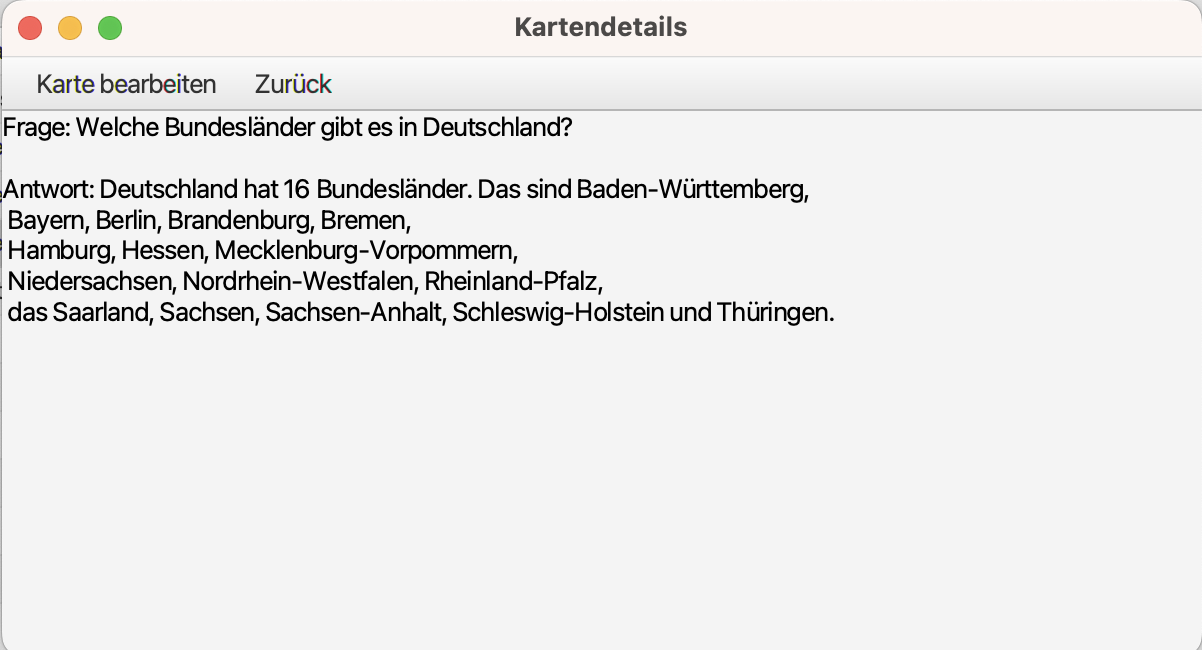
\includegraphics[width=\textwidth]{overview-details3.png}
\end{figure}

\begin{figure}
	\centering
	\caption{Dropdown Client-Einstellugen}
	\label{fig:settings}
	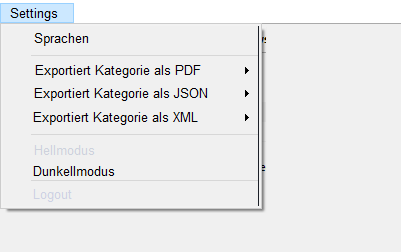
\includegraphics[width=0.6\textwidth]{settings.png}
\end{figure}


\end{document}
